\documentclass{article}%
\usepackage[T1]{fontenc}%
\usepackage[utf8]{inputenc}%
\usepackage{lmodern}%
\usepackage{textcomp}%
\usepackage{lastpage}%
\usepackage{authblk}%
\usepackage{graphicx}%
%
\title{Sparstolonin B, a Novel Plant Derived Compound, Arrests Cell Cycle and Induces Apoptosis in N{-}Myc Amplified and N{-}Myc Nonamplified Neuroblastoma Cells}%
\author{Tonya Moreno}%
\affil{Department of Oral and Maxillofacial Surgery, Hyogo College of Medicine, Nishinomiya, Hyogo 663{-}8501, Japan, Department of Genetics, Hyogo College of Medicine, Nishinomiya, Hyogo 663{-}8501, Japan}%
\date{01{-}01{-}2010}%
%
\begin{document}%
\normalsize%
\maketitle%
\section{Abstract}%
\label{sec:Abstract}%
Who the heck is Tenacibaculum? We probably dont need to point that out because it looks very much like a giant chocolate ice cream.\newline%
It was officially introduced in 2001 and underwent very little scientific rigour until 2007 when they made a number of changes to it, such as a specific class of expressions identified as softening effect. It is capable of changing in an appropriate sequence during the introductory stages of its development, with important impacts eventually contributing to vaccine success.\newline%
It is one of the most difficult vaccines to develop, taking several years and testing four times for a number of reasons. However, it has been made the subject of some exciting and interesting work and, now that it is more established, can finally be made available for purchase for consumers.\newline%
About its author: Dr. Naseem Farooq is a recognised expert on vaccination and epidemiology, practising ecologist and a geneticist at Government Medical College and Hospital, Republic of Lahore, Pakistan. He is also founder of Foundation for Research and Surveillance of Infectious Diseases, Executive Director of the National Rural Health Programme, Chairman of the Infectious Diseases Coordination Advisory Council of Lahore University of Management Sciences, Lahore, Chairman of the European Union Collaborative on Hepatitis, Research and Virospital of Research in Bt Vaccines in Asia, Non{-}Population Health Central Committee (CRC), and the Director of the National Institute of Allergy and Infectious Diseases, Iqbal Sadiq. He has been published for thirty years on Population Protection and Infectious Diseases, polio vaccine and pediatric immunization. In 2008, he was recognised by British Columbia Cancer Agency as a fellow of the Royal Society of British Medicine.

%
\subsection{Image Analysis}%
\label{subsec:ImageAnalysis}%


\begin{figure}[h!]%
\centering%
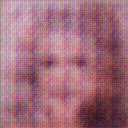
\includegraphics[width=150px]{500_fake_images/samples_5_398.png}%
\caption{A Black And White Photo Of A Zebra}%
\end{figure}

%
\end{document}